% Copyright 2013 by Mark Wibrow
%
% This file may be distributed and/or modified
%
% 1. under the LaTeX Project Public License and/or
% 2. under the GNU Free Documentation License.
%
% See the file doc/generic/pgf/licenses/LICENSE for more details.


\section{Math Library}
\label{section-library-math}

\begin{tikzlibrary}{math}
    This library defines a simple mathematical language to define simple
    functions and perform sequences of basic mathematical operations.
\end{tikzlibrary}
%
\begin{codeexample}[setup code,hidden]
    \usetikzlibrary{math}
\end{codeexample}


\subsection{Overview}

\pgfname\ and \tikzname\ both use the \pgfname\ mathematical engine which
provides many commands for parsing expressions. Unfortunately the \pgfname\
math engine is somewhat cumbersome for long sequences of mathematical
operations, particularly when assigning values to multiple variables. The
\tikzname\ |calc| library provides some additional ``convenience'' operations
for doing calculations (particularly with coordinates), but this can only be
used inside \tikzname\ path commands.

This |math| library provides a means to perform sequences of mathematical
operations in a more `user friendly' manner than the \pgfname\ math engine. In
addition, the coordinate calculations of the |calc| library can be accessed
(provided it is loaded).
%
However as the |math| library uses the \pgfname\ math engine -- which uses pure
\TeX\ to perform all its calculations -- it is subject to the same speed and
accuracy limitations. It is worth bearing this in mind, before trying to
implement algorithms requiring intensive and highly accurate computation. You
can, of course use the |fp| or the |fpu| libraries to increase the accuracy
(but not necessarily the speed) of computations.

For most purposes, the features provided by this library are accessed using the
following command:

\begin{command}{\tikzmath\texttt{\{}\meta{statements}\texttt{\}}}
    This command process  a series of \meta{statements} which can represent
    assignments, function definitions, conditional evaluation, and iterations.
    It provides, in effect, a miniature mathematical language to perform basic
    mathematical operations. Perhaps the most important thing to remember is
    that \emph{every statement should end with a semi-colon}. This is likely to
    be the most common reason why the |\tikzmath| command fails.
    %
\begin{codeexample}[]
\tikzmath{
  % Adapted from http://www.cs.northwestern.edu/academics/courses/110/html/fib_rec.html
  function fibonacci(\n) {
    if \n == 0 then {
      return 0;
    } else {
       return fibonacci2(\n, 0, 1);
     };
  };
  function fibonacci2(\n, \p, \q) {
    if \n == 1 then {
      return \q;
    } else {
      return fibonacci2(\n-1, \q, \p+\q);
    };
  };
  int \f, \i;
  for \i in {0,1,...,20}{
    \f = fibonacci(\i);
    print {\f, };
  };
}
\end{codeexample}
    %
\end{command}

In addition to this command the following key is provided:

\begin{key}{/tikz/evaluate={\meta{statements}}}
    This key simply executes |\tikzmath{|\meta{statements}|}|.
    %
\begin{codeexample}[]
\tikz[x=0.25cm,y=0.25cm,
  evaluate={
    int \i, \j;
    for \i in {0,...,10}{
      for \j in {0,...,10}{
        \a{\i,\j} = (\i+\j)*5;
      };
    };
  }
]
\foreach \i in {0,...,10}
  \foreach \j in {0,...,10}
    \fill [red!\a{\i,\j}!yellow]  (\i,\j) rectangle ++(1, 1);

\end{codeexample}
    %
\end{key}

The following sections describe the miniature language that this library
provides and   can be used in the |\tikzmath| command and the |evaluate| key.
The language consists only of simple keywords and expressions but the
mini-parser allows you to format code in a reasonably versatile way (much like
the |tikz| parser) except that \emph{all the keywords must be followed by at
least one space}. This is the second most important thing to remember (after
remembering to insert semi-colons at the end of every statement).


\subsection{Assignment}

In the simplest case, you will want to evaluate an expression and assign it to
a macro, or a \TeX\ count or dimension register. In this case, use of the
|math| library is straightforward:
%
\begin{codeexample}[]
\newcount\mycount
\newdimen\mydimen
\tikzmath{
  \a = 4*5+6;
  \b = sin(30)*4;
  \mycount = log10(2048) / log10(2);
  \mydimen = 15^2;
}
\a, \b, \the\mycount, \the\mydimen
\end{codeexample}

In addition, \TeX-macros (\emph{not} \TeX\ registers) can be suffixed with an
index, similar to indices in mathematical notation, for example, $x_1$, $x_2$,
$x_3$:
%
\begin{codeexample}[]
\tikzmath{
  \x1 = 3+4; \x2 = 30+40; \x3 = 300+400;
}
\x1, \x2, \x3
\end{codeexample}

The index does not have to be a number. By using braces |{}|, more
sophisticated indices can be created:
%
\begin{codeexample}[]
\tikzmath{
  \c{air} = 340; \c{water} = 1435; \c{steel} = 6100;
}
\foreach \medium in {air,steel}{The speed of sound in \medium\ is \c{\medium} m/s. }
\end{codeexample}

You should not, however, try to mix indexed and non-indexed variables. Once an
assignment is made using an index, the |math| library expects all instances of
the variable on the right hand side of an assignment to be followed by an
index. This effect is reversed if you subsequently make an assignment to the
variable without an index: the |math| library (or to be precise the \pgfname\
math-engine) will then ignore any index following the variable on the right
hand side of an assignment.

In some cases, you may wish to assign a value or expression to a variable
without evaluating it with the \pgfname\ math-engine. In this case, you can use
the following keyword:

\begin{math-keyword}{{let} \meta{variable} \texttt{=} \meta{expression}\texttt{;}}
    This keyword assigns \meta{expression} to \meta{variable} without
    evaluation. The \meta{expression} is however fully expanded using |\edef|.
    Any spaces preceding \meta{expression} are removed, but any trailing spaces
    (before the semi-colon) are included.
    %
\begin{codeexample}[]
\tikzmath{
  let \x = (5*4)+1;
  let \c1 = blue;
}
\x, ``\c1''
\end{codeexample}
    %
\end{math-keyword}


\subsection{Integers, ``Real'' Numbers, and Coordinates}

By default, assignments are made by evaluating expressions using the \pgfname\
math-engine and results  are usually returned as number with a decimal point
(unless you are assigning to a count register or use the |int| function).
%
As this is not always desirable, the |math| library allows variables -- which
\emph{must} be \TeX\ macros -- to be `declared' as being a particular `type'.
The library recognizes three types: integers (numbers without a decimal point),
real numbers (numbers with a decimal point\footnote{Strictly speaking, due to
the finite range and precision of \TeX\ numerical capabilities, the term
``real'' is not correct.}), and coordinates.

To declare a variable as being one of the three types, you  can use the
keywords shown below. It is important to remember that by telling the |math|
library you want it to do a particular assignment for a variable, it will also
do the same assignment when the variable is indexed.
%
\begin{codeexample}[]
\tikzmath{
  integer \x;
  \x1 = 3+4; \x2 = 30+40; \x3 = 300+400;
}
\x1, \x2, \x3
\end{codeexample}

%But, if you want integer results without using a count register or the
%|int| function, you can use a keyword to indicate this:

\begin{math-keyword}{{integer} \meta{variable}\opt{\texttt{,} \meta{additional variables}}\texttt{;}}
    The |integer| keyword indicates that assignments to the \meta{variable} or
    the comma separated list of \meta{additional variables} should be truncated
    (not rounded) to integers. The variables should be ordinary macros --
    \emph{not} \TeX\ registers. In addition the variables should \emph{not} be
    indexed.
    %
\begin{codeexample}[]
\tikzmath{
   integer \x, \y, \z;
   \x = 4*5+6;
   \y = sin(30)*4;
   \z = log10(512) / log10(2);
   print {$x=\x$, $y=\y$, $z=\z$};
}
\end{codeexample}
    %
\end{math-keyword}

\begin{math-keyword}{{int} \meta{variable}\opt{\texttt{,} \meta{additional variables}}\texttt{;}}
    Short version of the |integer| keyword.
\end{math-keyword}

Having declared a variable as an integer, the |math| library will continue to
assign only integers to that variable within the current \TeX\ scope. If you
wish to assign non-integer (i.e., \emph{real}) numbers to the same variable,
the following keyword can be used.

\begin{math-keyword}{{real} \meta{variable}\opt{\texttt{,} \meta{additional variables}}\texttt{;}}
    The |real| keyword ensures that assignments \meta{variable} (and
    \meta{additional variables}) will not be truncated to integers.
\end{math-keyword}

In order to take advantage of |math| library interface to the |calc| library
you must indicate that a variable is to be assigned coordinates, using the
following keyword.

\begin{math-keyword}{{coordinate} \meta{variable}\opt{\texttt{,} \meta{additional variables}}\texttt{;}}
    This keyword enables \tikzname-style coordinates such as |(2cm,3pt)| or
    |(my node.east)| to be parsed and assigned to \meta{variable} in the form
    $x,y$, which can then be used in a |tikzpicture|:
    %
\begin{codeexample}[]
\tikzmath{
   coordinate \c;
   \c = (45:10pt);
}
\tikz\draw (0,0) -- (\c);
\end{codeexample}

    If the \tikzname\ |calc| library is loaded, coordinate calculations can be
    performed; the coordinate expression does not have to be surrounded by
    |($|\ldots|$)|.
    %
\begin{codeexample}[]
\tikzmath{
   coordinate \c, \d;
   \c = (-1,2)+(1,-1);
   \d = (4,1)-(2,-1);
}
\tikz\draw (\c) -- (\d);
\end{codeexample}

    In addition to assigning the $x$ and $y$ coordinates to \meta{variable}
    (possibly with an optional index), two further variables are defined. The
    first takes the name of \meta{variable} (e.g., |\c|) suffixed with |x|
    (i.e., |\cx|) and is assigned the $x$ coordinate of |\c|. The second takes
    the name of \meta{variable} suffixed with |y| (i.e., |\cy|) and is assigned
    the $y$ coordinate of |\c|.
    %
\begin{codeexample}[]
\tikzmath{
   coordinate \c;
   \c1 = (30:20pt);
   \c2 = (210:20pt);
}
\tikz\draw (\cx1,\cy1) -- (\cx2,\cy1) -- (\cx2,\cy2) -- (\cx1,\cy2);
\end{codeexample}
    %
\end{math-keyword}

%\begin{math-keyword}{{point} \meta{variable}\opt{\texttt{,} \meta{additional variables}}\texttt{;}}
%    The |point| keyword is a synonym for the |coordinate| keyword and performs
%    the same function.
%\end{math-keyword}


\subsection{Repeating Things}

\begin{math-keyword}{{for} \meta{variable} \texttt{in \{}\meta{list}\texttt{\}\{}\meta{expressions}\texttt{\};}}
    This is a ``trimmed down'' version of the |\foreach| command available as
    part of \pgfname\ and \tikzname, but cannot currently be used outside of
    the |\tikzmath| command. It is important to note the following:
    %
    \begin{itemize}
        \item Every value in \meta{list} is evaluated using the \pgfname\
            mathematical engine. However, if an item in \meta{list} contains a
            comma, it \emph{must} be surrounded by braces, for example,
            |{mod(5, 2)}|.
            %
\begin{codeexample}[]
\tikzmath{
  int \x, \v;
  \v=1;
  for \x in {1,...,{random(3,10)}}{
     \v=\v*2;
  };
  print {$x=\x, v=\v$};
}
\end{codeexample}
            %
        \item Because each item is evaluated, you cannot use \tikzname\
            coordinates in \meta{list}.
        \item Only single variable assignment is supported.
        \item The ``dots notation'' (e.\,g., |1,2,...,9|) can be used in
            \meta{list}, but is not as sophisticated as the \pgfname\
            |\foreach| command. In particular, contextual replacement is not
            possible.
        \item Assignments that occur in the loop body \emph{are not scoped}.
            They last beyond the body of each iteration and the end of the
            |for| statement. This includes the values assigned to the
            \meta{variable}.
            %
\begin{codeexample}[]
\tikzmath{
  int \x, \y;
  \y = 0;
  for \x1 in {1,...,5}{
    for \x2 in {10,20,...,50}{
      \y = \y+\x1*\x2;
    };
  };
}
$x_1=\x1, x_2=\x2, y=\y$
\end{codeexample}
    \end{itemize}
\end{math-keyword}


\subsection{Branching Statements}

Sometimes you may wish to execute different statements depending on the value
of an expression. In this case the following keyword can be used:

\begin{math-keyword}{{if} \meta{condition} \texttt{then \{}\meta{if-non-zero-statements}\texttt{\};}}
    This keyword executes \meta{if-non-zero-statements} if the expression in
    \meta{condition} evaluates to any value other than zero.
\end{math-keyword}

\begin{math-keyword}{{if} \meta{condition} \texttt{then \{}\meta{if-non-zero-statements}\texttt{\}} \texttt{else} \texttt{\{}\meta{if-zero-statements}\texttt{\}}\texttt{;}}
    This keyword executes \meta{if-non-zero-statements} if the expression in
    \meta{condition} evaluates to any value other than zero and the
    \meta{if-zero-statements} are executed if the expression in
    \meta{condition} evaluates to zero.
    %
\begin{codeexample}[]
  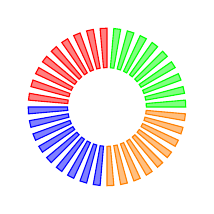
\begin{tikzpicture}
  \tikzmath{
    int \x;
    for \k in {0,10,...,350}{
      if \k>260 then { let \c = orange; } else {
        if \k>170 then { let \c = blue; } else {
          if \k>80 then { let \c = red; } else {
            let \c = green; }; }; };
      {
        \path [fill=\c!50, draw=\c] (\k:0.5cm) -- (\k:1cm) --
          (\k+5:1cm) -- (\k+5:0.5cm) -- cycle;
      };
    };
  }
  \end{tikzpicture}
\end{codeexample}
    %
\end{math-keyword}


\subsection{Declaring Functions}

You can add functions by using the following keywords:

\begin{math-keyword}{{function} \meta{name}\texttt{(}\meta{arguments}\texttt{) \{} \meta{definition} \texttt{\};}}
    This keyword works much like the |declare function| provided by the
    \pgfname\ math-engine. The function \meta{name} can be any name that is not
    already a function name in the current scope. The list of \meta{arguments}
    are comma separated \TeX\ macros such as |\x|, or |\y| (it is not possible
    to declare functions that take variable numbers of arguments). If the
    function takes no arguments then the parentheses need not be used. It is
    very important to note that the arrays that the \pgfname\ math engine
    supports \emph{cannot currently be passed as arguments to functions}.

    The function \meta{definition} should be a sequence of statements that can
    be parsed by the |\tikzmath| command and should use the commands specified
    in the \meta{arguments}. The |return| keyword (described below) should be
    used to indicate the value returned by the function.
    %
    Although \meta{definition} can take any statements accepted by |\tikzmath|,
    it is not advisable try to define functions inside other functions.
    %
\begin{codeexample}[]
\tikzmath{
  function product(\x,\y) {
    return \x*\y;
  };
  int \i, \i, \k;
  \i = random(1,10);
  \j = random(20, 40);
  \k = product(\i, \j);
  print { $\i\times \j = \k$ };
}
\end{codeexample}
    %
\end{math-keyword}

\begin{math-keyword}{{return} \meta{expression}\texttt{;}}
    This keyword should be used as the last executed statement in a function
    definition to indicate the value that should be returned.
\end{math-keyword}


\subsection{Executing Code Outside the Parser}

Sometimes you may wish to do ``something'' outside the parser, perhaps display
some intermediate result or execute some code. In this case you have two
options. Firstly, the following keyword can be used:

\begin{math-keyword}{{print} \texttt{\{}\meta{code}\texttt{\};}}
    Execute \meta{code} immediately. This is intended as convenience keyword
    for displaying information in a document (analogous to the |print| command
    in real programming languages). The \meta{code} is executed inside a \TeX\
    group.
    %
\begin{codeexample}[]
\tikzmath{
  int \x, \y, \z;
  \x = random(2, 5);
  for \y in {0,...,6}{
    \z = \x^\y;
    print {$\x^\y=\z$, };
  };
}
\end{codeexample}
    %
\end{math-keyword}

Secondly, if a statement begins with  a brace |{|, then everything up to the
closing brace |}| is collected and executed (the closing brace \emph{must} be
followed by a semi-colon). Like the |print| keyword, the contents of the braces
is executed inside a \TeX\ group. Unlike the |print| keyword, the brace
notation can be used in functions so that |tikz| path commands can be safely
executed inside a |tikzpicture|.
%
\begin{codeexample}[]
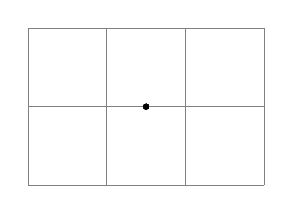
\begin{tikzpicture}
\draw [help lines] grid (3,2);
\tikzmath{
  coordinate \c;
  for \x in {0,10,...,360}{
    \c = (1.5cm, 1cm) + (\x:1cm and 0.5cm);
    { \fill (\c) circle [radius=1pt]; };
  };
}
\end{tikzpicture}
\end{codeexample}
